\section{Subsistema: Estrutura}
As dimensões do carrinho foram feitas com base na ergonomia utilizando uma cadeira de rodas como base. A altura máxima do carrinho será de 800mm para que o cadeirante tenha facilidade de colocar e retirar os objetos nele.

\par As dimensões da cesta foram de 800mm de comprimento, 500mm de largura e 250mm de profundidade. Os 500mm de largura levou em consideração a largura da cadeira de rodas. Essa largura permite que o carrinho esteja atrás do cadeirante sem que ocupe um espaço maior que o da cadeira no corredor. O comprimento e a profundidade foram com base no volume de 100L que o carrinho será capaz de transportar e levando em consideração a capacidade do cadeirante de retirar objetos sem dificuldades.

\par Na base do carrinho será uma chapa de alumínio onde serão fixados os motores, as rodas e as baterias, sendo necessário a fabricação de suportes. Ele possuirá quatro suportes que irão unir a base e a cesta do carrinho.

%2 imagens
 \begin{figure}[ht]
		\centering
		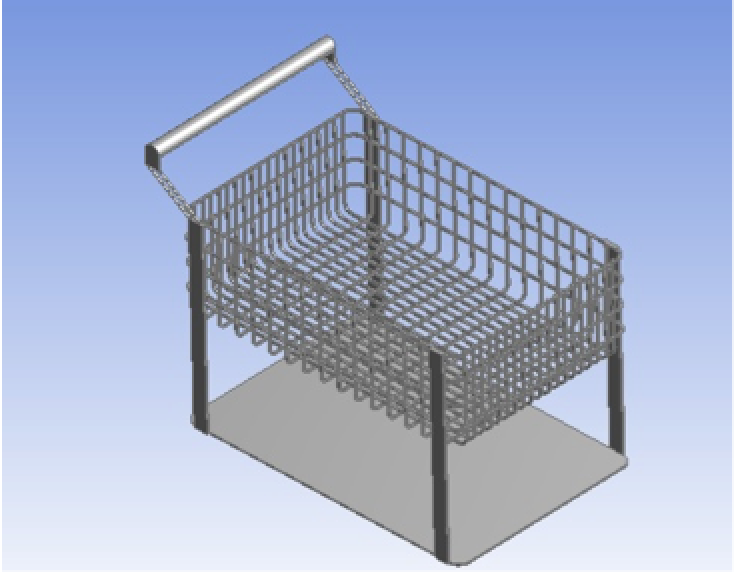
\includegraphics[width=.4\textwidth]{figuras/CADcarrinho.png}
		\caption{CAD da estrutura do carrinho}
		\label{fig:CADcarrinho}
	\end{figure} 
    
 \begin{figure}[ht]
		\centering
		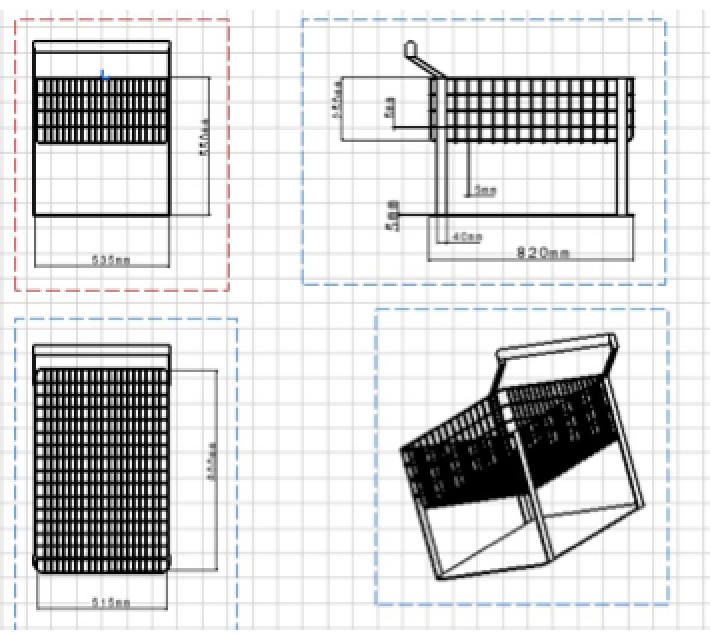
\includegraphics[width=.4\textwidth]{figuras/estrutura.png}
		\caption{Dimensões da estrutura do carrinho}
		\label{fig:estrutura}
	\end{figure} 

\par Foi escolhido o alumínio para ser usado na estrutura, pois o carrinho estará em uso constante nos supermercados, comportando um peso considerável e sofrendo vibração devido ao atrito com o piso conforme onde este é usado. Qualquer ação diária faz com que o carrinho sofra desgastes e se o material for frágil ele se danificará facilmente.

\par O alumínio é leve e resistente, pesando 1/3 do peso do aço, possuindo densidade de $2.7\frac{g}{cm^3}$ . O peso baixo do alumínio é uma vantagem para a aplicação no carrinho, pois diminui o peso total do carrinho, diminuindo assim a força necessária para movimentar o carrinho.

\par Este é altamente resistente a corrosão, por ter uma camada protetora de oxido.

%imagem
 \begin{figure}[ht]
		\centering
		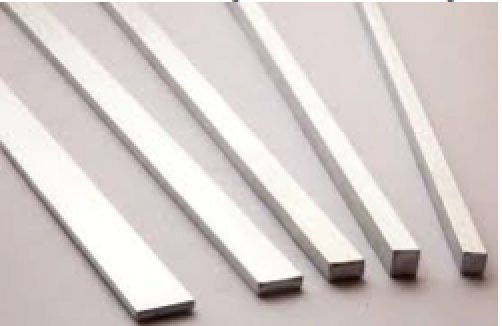
\includegraphics[width=.4\textwidth]{figuras/barrasaluminio.png}
		\caption{Barras de alumínio}
		\label{fig:barrasaluminio}
	\end{figure} 

\subsection{Rodas}
O ideal é que o equipamento disponha de rodas de aço e giratórias, que deslizam com facilidade, independente do tipo de piso, funcionando bem tanto para um piso liso, como o do mercado, como para um piso com rugosidade, igual do estacionamento do mercado, precisando assim de uma rodinha que não se danifique por conta do dele.

%imagem
 \begin{figure}[ht]
		\centering
		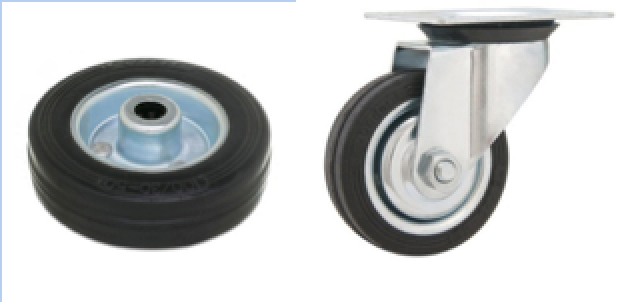
\includegraphics[width=.4\textwidth]{figuras/roda.png}
		\caption{Rodinha com e sem rodízio}
		\label{fig:roda}
	\end{figure} 

\par As rodas traseiras e dianteiras serão com rodizio, tendo diâmetro de 101 mm e largura de 27mm de largura, resistindo um peso 60kg por rodinha.

\subsection{Transmissão}

O uso da transmissão irá depender do motor utilizado no projeto, caso o motor não possua torque necessário para movimentar o carrinho, será necessário uma transmissão para aumentar o torque que entra na roda traseira do carrinho.
	
\par Existem diversos tipos de elementos que são utilizados para fazer a transmissão da potência do motor para as rodas, como por exemplo as correias, as correntes e as engrenagens. Em alguns casos, elas simplificam o projeto, reduzindo assim o custo \cite{Projmec}.

\subsection{Correias}
Existem quatro tipos de correias: as correias planas, que utilizam polias coroadas; correias redondas, que utilizam polias ranhuradas ou acanaladas; correias em V, que utilizam os mesmos tipos de polias das correias redondas; correias de tempo, que utilizam rodas dentadas, ou catracas.
	
\par Os eixos precisam ser separados por uma distância mínima, dependendo da correia e do seu tamanho, para que assim esta possa trabalhar apropriadamente. As correias podem ser utilizadas para longas distâncias de centro.

%imagem
 \begin{figure}[ht]
		\centering
		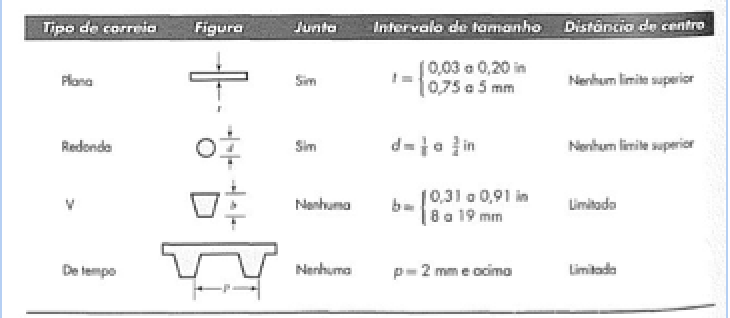
\includegraphics[width=.6\textwidth]{figuras/correia.png}
		\caption{Modelos de correia}
		\label{fig:correia}
	\end{figure} 

\textbf{1. Correias planas:}
Os materiais utilizados na fabricação de correias planas são o uretano e tecido impregnado de borracha reforçado com cordas de náilon ou de aço para absorver cargas de tensão.	

\par São silenciosas, e bastante eficiente em altas velocidades, podendo transmitir altas potências por longas distâncias entre centros.

\par As correrias planas possuem uma eficiência de 98\%, valor aproximado de uma transmissão por engrenagens

\par Normalmente, a correia plana é adquirida por rolo e depois cortada. As extremidades são unidas utilizando de apetrechos fornecidos pelo próprio fabricante.

\textbf{2. Correias em V:}
Os materiais utilizados na fabricação de correias em V são tecido, corda (de algodão, náilon ou raiom) e impregnada de borracha.
    
\par As correias em V são menos eficientes, quando comparadas às correias planas, possuindo uma eficiência entre 70 a 96\%.

\par São produzidas apenas em determinados tamanhos, não possuindo juntas.

\par Apresentam menor vibração, devido ao melhor balanço

\textbf{3. Correias de tempo:}
Algumas características das correias de tempo:

\begin{itemize}
\item Os materiais utilizados na fabricação das correias de tempo são tecido emborrachado e cabo de aço;
\item Não necessita de uma tensão inicial;
\item Possuem dentes para encaixar nas rodas dentadas;
\item Não estica e nem desliza, dessa maneira ela consegue transmitir potência com razão constante de velocidade angular;
\item Possui desvantagens no custo e nas flutuações dinâmicas que ocorrem no engrenamento da correia com as rodas dentadas;
\item Possui uma eficiência de 97 a 99\%;
\item Podem trabalhar em velocidades altas;
\item Não necessita de lubrificação;
\item Mais silenciosas do que transmissões feitas por corrente.
\end{itemize}

\textbf{4. Corrente de rolos:}
Algumas características das correntes de rolo:
    
\begin{itemize}
\item Possui uma razão constante, sem deslizamento e com vida longa;
\item Para que esta funcione de forma suave em velocidades moderadas ou altas, é recomendado o uso de uma roda dentada com pelo menos 17 dentes;
\item Para velocidades baixas, pode-se utilizar menores quantidades de dentes, porém isto diminui o tempo de vida da corrente;
\item Necessário lubrificação.
\end{itemize}

%imagem
 \begin{figure}[ht]
		\centering
		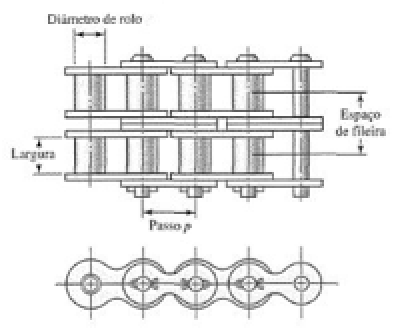
\includegraphics[width=.4\textwidth]{figuras/corrente.png}
		\caption{Correntes de rolo}
		\label{fig:corrente}
	\end{figure} 

\subsection{Engrenagens}
As forças transmitidas pelas engrenagens quando estas estão engrazadas geram momentos torcionais, gerando movimento e a transmissão da potência.

\par Para que ser transmitida essa potência, é necessário que as engrenagens tenham uma ação conjugada, onde a razão entre as velocidades angulares deve ser constante

\par Existem diversas maneiras para se fabricar dentes de engrenagens, como por exemplo a fundição em areia, fundição de investimento, fundição em molde permanente, moldagem em casa, entre outros \cite{Projmaq}.

\textbf{1. Engrenagens de dentes retos:}
Possuem dentes retos e são utilizadas para transmitir movimento, sendo que os eixos devem estar em paralelo um com o outro, sendo o modelo mais simples de engrenagens.
%imagem
\begin{figure}[ht]
		\centering
		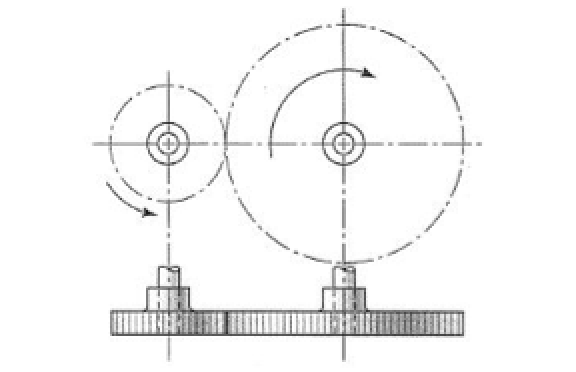
\includegraphics[width=.4\textwidth]{figuras/reto.png}
		\caption{Engrenagem de dente reto }
		\label{fig:reto}
	\end{figure}


\textbf{2. Engrenagens helicoidais:}
Possuem dentes inclinados em relação ao eixo, o qual ela rotaciona, podendo ser utilizada nas mesmas aplicações das engrenagens de dentes retos, porém não são tão barulhentas.
%imagem
\begin{figure}[ht]
		\centering
		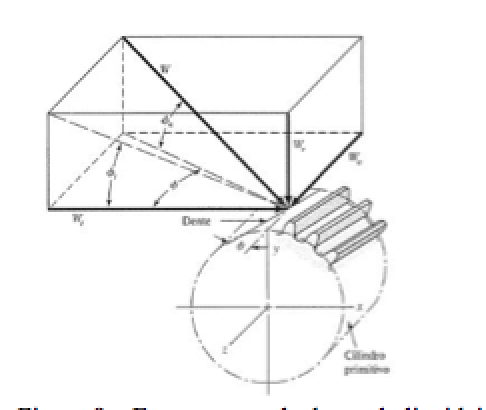
\includegraphics[width=.4\textwidth]{figuras/helicoidais.png}
		\caption{Engrenagem de dentes helicoidais}
		\label{fig:helicoidais}
	\end{figure}


\textbf{3. Engrenagens cônicas:}
Possuem dentes em uma superfície cônica, sendo utilizada para transmitir movimento entre eixos que se interceptam.
%imagem
\begin{figure}[ht]
		\centering
		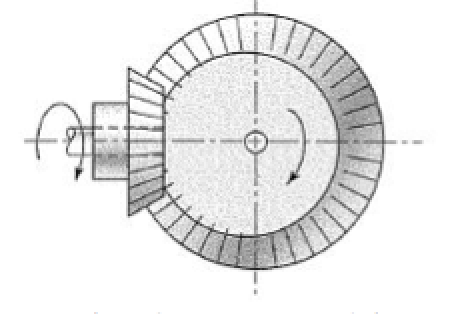
\includegraphics[width=.4\textwidth]{figuras/conica.png}
		\caption{Engrenagens cônicas }
		\label{fig:conica}
	\end{figure}

\par À partir desses modelos de transmissão, foi possível verificar que o provável modelo que será utilizado no projeto, será a correia plana, por ser mais silenciosa, por sua eficiência de 98\% e pela sua praticidade no ajuste de seu comprimento.

\subsection{Riscos associados}

Em todos projetos existem riscos. Dessa maneira, cabe a quem está projetando identificar as possíveis falhas que podem acontecer, para que se possa fazer uma planejamento de como evitar estas falhas. Para este projeto, podemos analisar a seguir, os seus possíveis riscos para o subsistema de estrutura:

\begin{itemize}
\item Estrutura do carrinho não resistir ao peso;
\item Rodinhas não resistirem aos esforços aplicados sobre ela;
\item Fabricação da estrutura do carrinho não ter sido feita corretamente ou não estar de acordo com o projeto;
\item Problemas físicos na transmissão;
\item Problemas na instalação de todos os componentes;
\item Tempo de aquisição dos matérias para fabricação e instalação.
\end{itemize}

\subsection{Cronograma físico-financeiro}
A estimativa de preços e aquisição para os recursos de estrutura foram estimados na tabela abaixo.

% ######## init table ########
\begin{table}[h]
 \centering
% distancia entre a linha e o texto
 {\renewcommand\arraystretch{1.25}
 \caption{Crononograma físico-financeiro Estrutura.}
 \begin{tabular}{ l l l }
  \cline{1-1}\cline{2-2}\cline{3-3}  
    \multicolumn{1}{|c|}{\textbf{Recurso} \centering } &
    \multicolumn{1}{c|}{\textbf{Data de aquisição} \centering } &
    \multicolumn{1}{c|}{\textbf{Estimativa de preço} \centering }
  \\  
  \cline{1-1}\cline{2-2}\cline{3-3}  
    \multicolumn{1}{|p{3.850cm}|}{Material para estrutura \centering } &
    \multicolumn{1}{p{4.217cm}|}{30/09 a 07/10/2016 \centering } &
    \multicolumn{1}{p{4.217cm}|}{R\$ 50,00 \centering }
  \\  
  \cline{1-1}\cline{2-2}\cline{3-3}  
    \multicolumn{1}{|p{3.850cm}|}{Rodas \centering } &
    \multicolumn{1}{p{4.217cm}|}{30/09 a 07/10/2016 \centering } &
    \multicolumn{1}{p{4.217cm}|}{R\$ 150,00 \centering }
  \\  
  \cline{1-1}\cline{2-2}\cline{3-3}  
    \multicolumn{1}{|p{3.850cm}|}{Trasmissão \centering } &
    \multicolumn{1}{p{4.217cm}|}{30/09 a 07/10/2016 \centering } &
    \multicolumn{1}{p{4.217cm}|}{R\$ 100,00 \centering }
  \\  
  \cline{1-1}\cline{2-2}\cline{3-3}  
    \multicolumn{2}{|p{3.850cm}|}{Total \centering } &
    \multicolumn{1}{p{4.217cm}|}{R\$ 300,00 \centering }
  \\  
  \hline

 \end{tabular} }
\end{table}

\subsection{Cronograma de atividades}

A Tabela a seguir apresenta todas as atividades que serão realizadas pelo subgrupo de estrutura até a entrega final do produto.

\clearpage

% ######## init table ########
\begin{table}[H]
 \centering
% distancia entre a linha e o texto
 {\renewcommand\arraystretch{1.25}
 \label{tab:cronestr}
 \caption{Cronograma de atividades Estrutura.}
 \begin{tabular}{ l l l l l }
  \cline{1-1}\cline{2-2}\cline{3-3}\cline{4-4}\cline{5-5}  
    \multicolumn{1}{|p{3.867cm}|}{\textbf{Atividade} \centering } &
    \multicolumn{1}{p{1.700cm}|}{\textbf{Duração} \centering } &
    \multicolumn{1}{p{1.133cm}|}{\textbf{Data inicial} \centering } &
    \multicolumn{1}{p{0.967cm}|}{\textbf{Data Final} \centering } &
    \multicolumn{1}{p{1.833cm}|}{\textbf{Status} \centering }
  \\  
  \cline{1-1}\cline{2-2}\cline{3-3}\cline{4-4}\cline{5-5}  
    \multicolumn{1}{|p{3.867cm}|}{Fase 1} &
    \multicolumn{1}{p{1.700cm}|}{7 dias \centering } &
    \multicolumn{1}{p{1.133cm}|}{17/08 \centering } &
    \multicolumn{1}{p{0.967cm}|}{24/08 \centering } &
    \multicolumn{1}{p{1.833cm}|}{Realizado \centering }
  \\  
  \cline{1-1}\cline{2-2}\cline{3-3}\cline{4-4}\cline{5-5}  
    \multicolumn{1}{|p{3.867cm}|}{Definir a geometria do carrinho} &
    \multicolumn{1}{p{1.700cm}|}{1 dia \centering } &
    \multicolumn{1}{p{1.133cm}|}{19/08 \centering } &
    \multicolumn{1}{p{0.967cm}|}{19/08 \centering } &
    \multicolumn{1}{p{1.833cm}|}{Realizado \centering }
  \\  
  \cline{1-1}\cline{2-2}\cline{3-3}\cline{4-4}\cline{5-5}  
    \multicolumn{1}{|p{3.867cm}|}{Pesquisa de ergonimia} &
    \multicolumn{1}{p{1.700cm}|}{5 dias \centering } &
    \multicolumn{1}{p{1.133cm}|}{19/08 \centering } &
    \multicolumn{1}{p{0.967cm}|}{24/08 \centering } &
    \multicolumn{1}{p{1.833cm}|}{Realizado \centering }
  \\  
  \cline{1-1}\cline{2-2}\cline{3-3}\cline{4-4}\cline{5-5}  
    \multicolumn{1}{|p{3.867cm}|}{Pesquisa de material } &
    \multicolumn{1}{p{1.700cm}|}{5 dias \centering } &
    \multicolumn{1}{p{1.133cm}|}{ 19/08 \centering } &
    \multicolumn{1}{p{0.967cm}|}{24/08 \centering } &
    \multicolumn{1}{p{1.833cm}|}{Realizado \centering }
  \\  
  \cline{1-1}\cline{2-2}\cline{3-3}\cline{4-4}\cline{5-5}  
    \multicolumn{1}{|p{3.867cm}|}{Definir componentes estruturais} &
    \multicolumn{1}{p{1.700cm}|}{5 dias \centering } &
    \multicolumn{1}{p{1.133cm}|}{19/08 \centering } &
    \multicolumn{1}{p{0.967cm}|}{24/08 \centering } &
    \multicolumn{1}{p{1.833cm}|}{Realizado \centering }
  \\  
  \cline{1-1}\cline{2-2}\cline{3-3}\cline{4-4}\cline{5-5}  
    \multicolumn{1}{|p{3.867cm}|}{Definir cronograma} &
    \multicolumn{1}{p{1.700cm}|}{1 dia \centering } &
    \multicolumn{1}{p{1.133cm}|}{24/08 \centering } &
    \multicolumn{1}{p{0.967cm}|}{24/08 \centering } &
    \multicolumn{1}{p{1.833cm}|}{Realizado \centering }
  \\  
  \cline{1-1}\cline{2-2}\cline{3-3}\cline{4-4}\cline{5-5}  
    \multicolumn{1}{|p{3.867cm}|}{Fase 2} &
    \multicolumn{1}{p{1.700cm}|}{15 dias \centering } &
    \multicolumn{1}{p{1.133cm}|}{24/08 \centering } &
    \multicolumn{1}{p{0.967cm}|}{09/09 \centering } &
    \multicolumn{1}{p{1.833cm}|}{Realizado \centering }
  \\  
  \cline{1-1}\cline{2-2}\cline{3-3}\cline{4-4}\cline{5-5}  
    \multicolumn{1}{|p{3.867cm}|}{Fazer CAD inicial do carrinho} &
    \multicolumn{1}{p{1.700cm}|}{5 dias \centering } &
    \multicolumn{1}{p{1.133cm}|}{26/08 \centering } &
    \multicolumn{1}{p{0.967cm}|}{31/08 \centering } &
    \multicolumn{1}{p{1.833cm}|}{Realizado \centering }
  \\  
  \cline{1-1}\cline{2-2}\cline{3-3}\cline{4-4}\cline{5-5}  
    \multicolumn{1}{|p{3.867cm}|}{Pesquisa de modelo de rodinhas, transmissão e custos} &
    \multicolumn{1}{p{1.700cm}|}{5 dias \centering } &
    \multicolumn{1}{p{1.133cm}|}{26/08 \centering } &
    \multicolumn{1}{p{0.967cm}|}{31/08 \centering } &
    \multicolumn{1}{p{1.833cm}|}{Realizado \centering }
  \\  
  \cline{1-1}\cline{2-2}\cline{3-3}\cline{4-4}\cline{5-5}  
    \multicolumn{1}{|p{3.867cm}|}{Documentação} &
    \multicolumn{1}{p{1.700cm}|}{3 dis \centering } &
    \multicolumn{1}{p{1.133cm}|}{29/08 \centering } &
    \multicolumn{1}{p{0.967cm}|}{02/09 \centering } &
    \multicolumn{1}{p{1.833cm}|}{Realizado \centering }
  \\  
  \cline{1-1}\cline{2-2}\cline{3-3}\cline{4-4}\cline{5-5}  
    \multicolumn{1}{|p{3.867cm}|}{Apresentação} &
    \multicolumn{1}{p{1.700cm}|}{1 dia \centering } &
    \multicolumn{1}{p{1.133cm}|}{09/09 \centering } &
    \multicolumn{1}{p{0.967cm}|}{09/09 \centering } &
    \multicolumn{1}{p{1.833cm}|}{Realizado \centering }
  \\  
  \cline{1-1}\cline{2-2}\cline{3-3}\cline{4-4}\cline{5-5}  
    \multicolumn{1}{|p{3.867cm}|}{Fase 3} &
    \multicolumn{1}{p{1.700cm}|}{61 dias \centering } &
    \multicolumn{1}{p{1.133cm}|}{09/09 \centering } &
    \multicolumn{1}{p{0.967cm}|}{09/11 \centering } &
    \multicolumn{1}{p{1.833cm}|}{À fazer \centering }
  \\  
  \cline{1-1}\cline{2-2}\cline{3-3}\cline{4-4}\cline{5-5}  
    \multicolumn{1}{|p{3.867cm}|}{Pesquisa de processos de fabricação} &
    \multicolumn{1}{p{1.700cm}|}{5 dias \centering } &
    \multicolumn{1}{p{1.133cm}|}{09/09 \centering } &
    \multicolumn{1}{p{0.967cm}|}{14/09 \centering } &
    \multicolumn{1}{p{1.833cm}|}{À fazer \centering }
  \\  
  \cline{1-1}\cline{2-2}\cline{3-3}\cline{4-4}\cline{5-5}  
    \multicolumn{1}{|p{3.867cm}|}{Definir modelos de rodas e transmissão} &
    \multicolumn{1}{p{1.700cm}|}{12 dias \centering } &
    \multicolumn{1}{p{1.133cm}|}{02/09 \centering } &
    \multicolumn{1}{p{0.967cm}|}{14/09 \centering } &
    \multicolumn{1}{p{1.833cm}|}{À fazer \centering }
  \\  
  \cline{1-1}\cline{2-2}\cline{3-3}\cline{4-4}\cline{5-5}  
    \multicolumn{1}{|p{3.867cm}|}{Cálculos de transmissão} &
    \multicolumn{1}{p{1.700cm}|}{7 dias \centering } &
    \multicolumn{1}{p{1.133cm}|}{14/09 \centering } &
    \multicolumn{1}{p{0.967cm}|}{21/09 \centering } &
    \multicolumn{1}{p{1.833cm}|}{À fazer \centering }
  \\  
  \cline{1-1}\cline{2-2}\cline{3-3}\cline{4-4}\cline{5-5}  
    \multicolumn{1}{|p{3.867cm}|}{Pesquisa de mercado de transmissão e material} &
    \multicolumn{1}{p{1.700cm}|}{3 dias \centering } &
    \multicolumn{1}{p{1.133cm}|}{21/09 \centering } &
    \multicolumn{1}{p{0.967cm}|}{23/09 \centering } &
    \multicolumn{1}{p{1.833cm}|}{À fazer \centering }
  \\  
  \cline{1-1}\cline{2-2}\cline{3-3}\cline{4-4}\cline{5-5}  
    \multicolumn{1}{|p{3.867cm}|}{Simulação do CAD} &
    \multicolumn{1}{p{1.700cm}|}{11 dias \centering } &
    \multicolumn{1}{p{1.133cm}|}{28/09 \centering } &
    \multicolumn{1}{p{0.967cm}|}{07/10 \centering } &
    \multicolumn{1}{p{1.833cm}|}{À fazer \centering }
  \\  
  \cline{1-1}\cline{2-2}\cline{3-3}\cline{4-4}\cline{5-5}  
    \multicolumn{1}{|p{3.867cm}|}{Compra de recursos (material, rodinhas e transmissão)} &
    \multicolumn{1}{p{1.700cm}|}{8 dias \centering } &
    \multicolumn{1}{p{1.133cm}|}{30/09 \centering } &
    \multicolumn{1}{p{0.967cm}|}{07/10 \centering } &
    \multicolumn{1}{p{1.833cm}|}{À fazer \centering }
  \\  
  \cline{1-1}\cline{2-2}\cline{3-3}\cline{4-4}\cline{5-5}  
    \multicolumn{1}{|p{3.867cm}|}{Fabricação da estrutura e de suporte} &
    \multicolumn{1}{p{1.700cm}|}{17 dias \centering } &
    \multicolumn{1}{p{1.133cm}|}{21/10 \centering } &
    \multicolumn{1}{p{0.967cm}|}{28/10 \centering } &
    \multicolumn{1}{p{1.833cm}|}{À fazer \centering }
  \\  
  \cline{1-1}\cline{2-2}\cline{3-3}\cline{4-4}\cline{5-5}  
    \multicolumn{1}{|p{3.867cm}|}{Documentação dos avanços} &
    \multicolumn{1}{p{1.700cm}|}{5 dias \centering } &
    \multicolumn{1}{p{1.133cm}|}{21/10 \centering } &
    \multicolumn{1}{p{0.967cm}|}{28/10 \centering } &
    \multicolumn{1}{p{1.833cm}|}{À fazer \centering }
  \\  
  \cline{1-1}\cline{2-2}\cline{3-3}\cline{4-4}\cline{5-5}  
    \multicolumn{1}{|p{3.867cm}|}{Apresentação} &
    \multicolumn{1}{p{1.700cm}|}{1 dia \centering } &
    \multicolumn{1}{p{1.133cm}|}{09/11 \centering } &
    \multicolumn{1}{p{0.967cm}|}{09/11 \centering } &
    \multicolumn{1}{p{1.833cm}|}{À fazer \centering }
  \\  
  \cline{1-1}\cline{2-2}\cline{3-3}\cline{4-4}\cline{5-5}  
    \multicolumn{1}{|p{3.867cm}|}{Fase 4} &
    \multicolumn{1}{p{1.700cm}|}{23 dias \centering } &
    \multicolumn{1}{p{1.133cm}|}{09/11 \centering } &
    \multicolumn{1}{p{0.967cm}|}{02/12 \centering } &
    \multicolumn{1}{p{1.833cm}|}{À fazer \centering }
  \\  
  \cline{1-1}\cline{2-2}\cline{3-3}\cline{4-4}\cline{5-5}  
    \multicolumn{1}{|p{3.867cm}|}{Integração dos subsistemas} &
    \multicolumn{1}{p{1.700cm}|}{12 dias \centering } &
    \multicolumn{1}{p{1.133cm}|}{11/11 \centering } &
    \multicolumn{1}{p{0.967cm}|}{30/11 \centering } &
    \multicolumn{1}{p{1.833cm}|}{À fazer \centering }
  \\  
  \cline{1-1}\cline{2-2}\cline{3-3}\cline{4-4}\cline{5-5}  
    \multicolumn{1}{|p{3.867cm}|}{Documentação final} &
    \multicolumn{1}{p{1.700cm}|}{5 dias \centering } &
    \multicolumn{1}{p{1.133cm}|}{25/11 \centering } &
    \multicolumn{1}{p{0.967cm}|}{30/11 \centering } &
    \multicolumn{1}{p{1.833cm}|}{À fazer \centering }
  \\  
  \cline{1-1}\cline{2-2}\cline{3-3}\cline{4-4}\cline{5-5}  
    \multicolumn{1}{|p{3.867cm}|}{Apresentação final} &
    \multicolumn{1}{p{1.700cm}|}{1 dia \centering } &
    \multicolumn{1}{p{1.133cm}|}{02/10 \centering } &
    \multicolumn{1}{p{0.967cm}|}{02/12 \centering } &
    \multicolumn{1}{p{1.833cm}|}{À fazer \centering }
  \\  
  \hline

 \end{tabular} }
\end{table}


	



























